\documentclass[aspectratio=169,10pt]{beamer}
\usetheme{Madrid}
\usecolortheme{seahorse}
\usefonttheme{professionalfonts}

\setbeamertemplate{footline}[frame number]
\setbeamertemplate{navigation symbols}{}

\graphicspath{{figures/}}

\usepackage{amsmath,amssymb,amsthm}
\usepackage{graphicx}
\usepackage{listings}
\usepackage{xcolor}
\usepackage{booktabs}

\lstset{
  basicstyle=\ttfamily\scriptsize,
  numbers=left,
  numberstyle=\tiny,
  frame=single,
  backgroundcolor=\color{gray!7},
  commentstyle=\color{green!50!black}\itshape,
  keywordstyle=\color{blue!70!black}\bfseries,
  stringstyle=\color{orange!70!black},
  breaklines=true,
  showstringspaces=false,
  language=Python
}

\newcommand{\PP}{\mathbb{P}}
\newcommand{\EE}{\mathbb{E}}
\newcommand{\RR}{\mathbb{R}}
\newcommand{\1}{\mathbbm{1}}

\title[E-Values -- Ch.11]{Hypothesis Testing with E-Values}
\subtitle{Chapter 11: Combining E-Values and Using E-Values as Weights}
\author{Based on Ramdas \& Wang}
\date{}

\begin{document}

% ==========================================================================
\begin{frame}
\titlepage
\end{frame}

% ==========================================================================
\begin{frame}{Outline}
\tableofcontents
\end{frame}

% ==========================================================================
\section{Notation and roadmap}

\begin{frame}[allowframebreaks]{Notation you'll need}

\textbf{The big picture.} This chapter answers three practical questions:
\begin{enumerate}
\item If I have $K$ separate e-values for the \emph{same} hypothesis, what are \emph{all} the valid ways to combine them into one e-value? (Section 11.2)
\item If I have one e-value \emph{and} one p-value for the same hypothesis, how do I combine them? (Section 11.3)
\item Can an e-value be used as a ``weight'' that makes a p-value-based multiple testing procedure (like Benjamini--Hochberg) more powerful? (Section 11.4)
\end{enumerate}

\vspace{2mm}
\textbf{Key vocabulary:}

\begin{itemize}
\item \textbf{E-merging function.} A function $F:\RR_+^K \to \RR_+$ that takes $K$ e-values $E_1,\dots,E_K$ (for the same null hypothesis, possibly arbitrarily dependent) and outputs $F(E_1,\dots,E_K)$, which is guaranteed to again be a valid e-value: $\EE[F(E_1,\dots,E_K)] \le 1$ under the null, no matter the dependence structure.

\item \textbf{Admissible.} An e-merging function $F$ is admissible if no other valid e-merging function $G$ satisfies $G \ge F$ everywhere with $G \ne F$ somewhere. In words: you cannot uniformly improve on it. Admissible rules are the ``non-wasteful'' ones worth using.

\item \textbf{Cross-merging.} Combining one e-value $E$ and one p-value $P$ (for the \emph{same} hypothesis) into a single output, which may itself be an e-value or a p-value. Section 11.3 calls such a combining function a \emph{combiner}.

\item \textbf{E-value as weight.} In multi-hypothesis testing, if hypothesis $H_k$ has both a p-value $P_k$ and an e-value $E_k$, the quotient $P_k/E_k$ (capped at 1) behaves like a p-value that has been ``reweighted'' by $E_k$: large $E_k$ (evidence against $H_k$) loosens the effective threshold, small $E_k$ tightens it. Section 11.4 plugs these reweighted p-values into ordinary FDR procedures.

\framebreak

\textbf{Reminder from earlier chapters (Chapter 8).} The simplex
\[
\Delta_{K+1} = \left\{ \boldsymbol\lambda = (\lambda_0,\lambda_1,\dots,\lambda_K) \in \RR_+^{K+1} : \sum_{k=0}^K \lambda_k = 1 \right\}
\]
indexes a family of linear e-merging functions
\[
\mathbb{M}_{\boldsymbol\lambda}(e_1,\dots,e_K) := \lambda_0 + \sum_{k=1}^K \lambda_k e_k .
\]
Here $\lambda_0$ is a constant ``skepticism'' weight (it shrinks the output toward the trivial e-value $1$), and $\lambda_1,\dots,\lambda_K$ are weights on the individual e-values. This chapter's main goal in Section 11.2 is to prove that \emph{these are the only admissible e-merging functions} (Theorem 8.4, stated already in Chapter 8, proved here).

\end{frame}

% ==========================================================================
\section{11.1 Optimal transport duality}

\begin{frame}{11.1 Optimal transport: the one-sentence idea}

\textbf{Plain-language explanation.} Optimal transport asks: if you have one pile of sand shaped like distribution $\mu$ and want to reshape it into a pile shaped like distribution $\nu$, what is the cheapest way to move the grains, given a cost of moving a grain from $x$ to $y$? ``Cheapest'' is a genuine minimization over all valid ways of moving mass (\emph{couplings}); the dual question -- looking at it from the price side -- turns out to have an equivalent, often easier-to-compute, formula.

\vspace{2mm}
\textbf{Why it shows up here.} Both e-merging functions and p-merging functions must remain valid under \emph{arbitrary dependence} between the input e-values/p-values. Certifying a property ``for the worst-case dependence'' is exactly a question about the set of all joint distributions (couplings) with fixed marginals -- which is precisely multi-marginal optimal transport. We only need the tool, not the theory behind it; we state the duality result without proof.

\end{frame}

% ---------------------------------------------------------------------------
\begin{frame}{Setup: the operator $\bigoplus$ and the constraint set $D_F$}

Fix $K \ge 2$. Let $F:[0,\infty)^K \to \RR$ be a bounded Borel function -- this will be the ``target'' function we want to dominate. Let $\mathcal{B}$ be the set of Borel functions on $[0,\infty)$.

\begin{block}{Additive-separable upper bounds}
For $(\phi_1,\dots,\phi_K) \in \mathcal{B}^K$, define the ``sum-of-univariate-functions'' operator
\[
\left(\bigoplus_{k=1}^K \phi_k\right)(x_1,\dots,x_K) := \sum_{k=1}^K \phi_k(x_k), \qquad (x_1,\dots,x_K) \in [0,\infty)^K,
\]
and the collection of separable functions that dominate $F$:
\[
D_F = \left\{ (\phi_1,\dots,\phi_K) \in \mathcal{B}^K \;:\; \bigoplus_{k=1}^K \phi_k \ge F \right\}.
\]
\end{block}

\textbf{Intuition.} $D_F$ collects every way of writing an upper bound for $F$ as a sum of $K$ functions, each depending on only \emph{one} coordinate. This ``separable'' structure is exactly what shows up when we bound $\EE[F(E_1,\dots,E_K)]$ coordinate by coordinate.

\end{frame}

% ---------------------------------------------------------------------------
\begin{frame}{Lemma 11.1: optimal transport duality}

Let $\Gamma(\mu_1,\dots,\mu_K)$ be the set of all Borel measures on $\RR^K$ with marginal distributions $\mu_1,\dots,\mu_K$ (all the ways to ``glue together'' $K$ distributions into a joint one -- all possible dependence structures).

\begin{block}{Lemma 11.1 (optimal transport duality)}
For any bounded Borel $F:[0,\infty)^K \to \RR$ and distributions $\mu_1,\dots,\mu_K$ on $\RR$,
\[
\sup_{\pi \in \Gamma(\boldsymbol\mu)} \int F \, \mathrm{d}\pi \;=\; \inf_{\boldsymbol\phi \in D_F} \sum_{k=1}^K \int \phi_k \, \mathrm{d}\mu_k,
\tag{11.1}
\]
where in the infimum we only consider $\boldsymbol\phi$ with $\sum_{k=1}^K \int \phi_k \mathrm{d}\mu_k$ well-defined.
\end{block}

\textbf{Reading the formula.}
\begin{itemize}
\item Left side: the worst-case (largest) expectation of $F$ over \emph{every} possible joint dependence structure $\pi$ with the given marginals -- this is exactly ``what's the worst that arbitrary dependence can do to $\EE[F]$?''
\item Right side: the cheapest separable upper bound to $F$, priced out coordinate by coordinate against each marginal.
\item Extra regularity: if $F$ is upper semicontinuous, the infimum is attained, and $\phi_k$ can be chosen upper semicontinuous; if $F$ is decreasing and nonnegative, so can $\phi_k$ be; if $F\in[0,1]$, so can $\phi_k$.
\end{itemize}

\end{frame}

% ==========================================================================
\section{11.2 Admissible e-merging functions}

\begin{frame}{11.2 Intuition: what are we proving?}

\textbf{Goal.} Recall (from Chapter 8) that an e-merging function $F$ satisfies $\EE^{\PP}[F(E_1,\dots,E_K)] \le 1$ for \emph{every} choice of e-variables $E_1,\dots,E_K$ (each with $\EE[E_k]\le 1$), no matter how they are dependent. We want to show:

\begin{block}{Recalling Theorem 8.4}
For a function $F:\RR_+^K \to \RR_+$:
\begin{enumerate}
\item[(i)] If $F$ is an e-merging function, then $F \le \mathbb{M}_{\boldsymbol\lambda}$ for some $\boldsymbol\lambda \in \Delta_{K+1}$.
\item[(ii)] $F$ is an \emph{admissible} e-merging function if and only if $F = \mathbb{M}_{\boldsymbol\lambda}$ for some $\boldsymbol\lambda \in \Delta_{K+1}$.
\end{enumerate}
\end{block}

\textbf{Why this is a clean and satisfying answer.} It says: no matter how clever a merging rule you dream up, it can never beat some simple linear combination $\lambda_0 + \sum_k \lambda_k e_k$. And every point on the simplex $\Delta_{K+1}$ gives a genuinely different, genuinely admissible, merging rule. Statement (ii) follows immediately from (i) together with the easy fact that $\mathbb{M}_{\boldsymbol\lambda}$ itself is always a valid e-merging function -- so all the work is in proving (i).

\end{frame}

% ---------------------------------------------------------------------------
\begin{frame}{Warm-up: the case $K=1$ (Lemma 11.2)}

\textbf{Intuition first.} With a single input, an e-merging function is just a function $g$ of one e-variable that stays a valid e-variable. The claim is that $g$ must be dominated by an \emph{affine} function of $x$: you cannot do better than mixing a constant with the identity.

\begin{block}{Lemma 11.2}
Let $\theta \in [1,\infty)$ and $r \in \RR_+$. If $g:[0,\theta]\to\RR_+$ satisfies $\EE^\PP[g(E)] \le r$ for all e-variables $E$ taking values in $[0,\theta]$, then there exists $\lambda \in [0,1]$ such that
\[
g(x) \le r(1-\lambda+\lambda x) \quad \text{for } x \in [0,\theta]\cap\RR.
\]
\end{block}

\textbf{Proof sketch (the key idea).}
\begin{itemize}
\item WLOG $r=1$. First show $g(y)\le y$ for $y>1$: if not, a two-point variable putting mass $1/y$ on $y$ (mean $1$) would violate $\EE[g(E)]\le 1$. Also $g(x)\le 1$ for $x\le 1$.
\item Suppose no single $\lambda$ works. Define $\Lambda_0=\{\lambda: g(y)>(1-\lambda)+\lambda y \text{ some } y>1\}$ and $\Lambda_1 = \{\lambda: g(x) > (1-\lambda)+\lambda x \text{ some } x<1\}$. These intervals cover $[0,1]$, so (by a continuity/sup-inf argument) they must \emph{overlap} at some $\lambda_0$.
\item At that overlapping $\lambda_0$, pick violating points $x_0<1<y_0$ and build the two-point e-variable $X$ with $\PP(X=y_0) = (1-x_0)/(y_0-x_0)$, $\PP(X=x_0)=(y_0-1)/(y_0-x_0)$ (mean exactly $1$). A direct computation gives $\EE[g(X)] > 1$ -- a contradiction.
\end{itemize}

\end{frame}

% ---------------------------------------------------------------------------
\begin{frame}{Consequence of Lemma 11.2: no free lunch from transforming $E$}

\begin{block}{Practical takeaway ($r=1$, general form)}
If $g$ is a (dimension-1) e-merging function, there exists $\lambda\in[0,1]$ with
\[
g(x) \le (1-\lambda) + \lambda x \qquad \text{for all } x \ge 0.
\]
\end{block}

\textbf{Why this matters.} Suppose you are handed a single e-variable $E$ and, hoping to do better, you consider transforming it -- say $\sqrt{E}$ is also a valid e-variable for any $E$. Lemma 11.2 says $\sqrt{E}$ is \emph{dominated} by $(1-\lambda)+\lambda E$ for some $\lambda$ (here $\lambda = 1/2$ turns out to work). So transforming a single e-value can never uniformly beat a simple affine mix with the constant $1$. This is also \emph{why}, in sequential testing (Chapter 7), the only way to combine a new e-variable $E_t$ into a running e-process at each step is via $(1-\lambda_t) + \lambda_t E_t$ -- there is no other admissible option.

\end{frame}

% ---------------------------------------------------------------------------
\begin{frame}{Upper semicontinuous reduction (Lemma 11.3)}

\textbf{Why we need this.} The optimal transport duality (Lemma 11.1) gives its nicest guarantees (attained infimum, semicontinuous $\phi_k$) when the target function $F$ is upper semicontinuous (u.s.c.). Real e-merging functions need not be u.s.c., so we first replace $F$ by a u.s.c.\ ``majorant'' that is at least as good, and show that if we can dominate the majorant, we dominate $F$ too.

\begin{block}{Lemma 11.3}
If $F$ is an e-merging function, then its upper semicontinuous version
\[
F^*(\mathbf{e}) = \lim_{\varepsilon \downarrow 0} F(\mathbf{e}+\varepsilon\mathbf{1}), \qquad \mathbf{e} \in [0,\infty)^K,
\]
is also an e-merging function, and $F^* \ge F$.
\end{block}

\textbf{Proof idea.} Take e-variables $\mathbf{E}$; for rational $\varepsilon\in(0,1)$ build a perturbed vector $\mathbf{E}_\varepsilon = (\mathbf{E}+\varepsilon\mathbf{1})\1_{A_\varepsilon}$ using an independent event $A_\varepsilon$ with $\PP(A_\varepsilon)=1-\varepsilon$. One checks $\EE[\mathbf{E}_\varepsilon]\le\mathbf{1}$, so $F(\mathbf{E}_\varepsilon)$ has expectation $\le 1$; expanding gives $\EE[F(\mathbf{E}+\varepsilon\mathbf{1})] \le \frac{1-\varepsilon F(\mathbf{0})}{1-\varepsilon}$. Fatou's lemma as $\varepsilon\downarrow 0$ then gives $\EE[F^*(\mathbf{E})]\le 1$.

\end{frame}

% ---------------------------------------------------------------------------
\begin{frame}{Proof of Theorem 8.4, step 1: set up the transport problem}

By Lemma 11.3, it suffices to prove the bound for u.s.c.\ $F$. Fix $\theta \ge 1$, and let $\mathcal{M}_{\mathcal E}^\theta$ be the set of all distributions on $[0,\theta]$ with mean $\le 1$ (i.e., distributions of e-variables bounded by $\theta$).

\textbf{Step 1: rewrite the worst-case expectation as a sup-sup, then apply Lemma 11.1.} Since $F$ is bounded, nonnegative on $[0,\theta]^K$, and u.s.c.,
\[
\sup_{\boldsymbol\mu \in (\mathcal M_{\mathcal E}^\theta)^K} \; \sup_{\pi\in\Gamma(\boldsymbol\mu)} \int F\,\mathrm{d}\pi
\;=\; \sup_{\boldsymbol\mu \in (\mathcal M_{\mathcal E}^\theta)^K} \; \inf_{\boldsymbol\phi \in D_F^+} \sum_{k=1}^K \int \phi_k \,\mathrm{d}\mu_k,
\tag{11.2}
\]
where $D_F^+ \subseteq D_F$ restricts to nonnegative, u.s.c.\ components (available thanks to the regularity clauses of Lemma 11.1).

\textbf{Interpretation.} The left side is: over every joint law $\pi$ of $K$ e-variables (any dependence, any marginals bounded by $\theta$), what's the worst-case value of $\EE[F(\mathbf E)]$? Since $F$ is an e-merging function, this worst case must be $\le 1$ -- that is the constraint we will exploit.

\end{frame}

% ---------------------------------------------------------------------------
\begin{frame}{Proof of Theorem 8.4, step 2: swap sup and inf (minimax)}

We now want to swap the order of $\sup_{\boldsymbol\mu}$ and $\inf_{\boldsymbol\phi}$ in (11.2). Define $J(\boldsymbol\mu,\boldsymbol\phi) = \sum_{k=1}^K \int \phi_k\,\mathrm{d}\mu_k$, and check three conditions for a minimax theorem (Fan, 1953):

\begin{enumerate}
\item[(i)] $J$ is \textbf{bilinear} in $(\boldsymbol\mu,\boldsymbol\phi)$, hence convex in $\boldsymbol\phi$ and concave in $\boldsymbol\mu$.
\item[(ii)] $[0,\theta]$ is compact, so $(\mathcal M_{\mathcal E}^\theta)^K$ (weak topology) is tight, hence (Prokhorov) sequentially compact, hence compact.
\item[(iii)] Each $\phi_k$ u.s.c.\ $\Rightarrow$ $\boldsymbol\mu \mapsto J(\boldsymbol\mu,\boldsymbol\phi)$ is u.s.c.\ in $\boldsymbol\mu$ (weak convergence) for each fixed $\boldsymbol\phi$.
\end{enumerate}

These conditions license Fan's minimax theorem:
\[
\sup_{\boldsymbol\mu\in(\mathcal M_{\mathcal E}^\theta)^K} \inf_{\boldsymbol\phi\in D_F^+} \sum_{k=1}^K \int\phi_k\mathrm{d}\mu_k
= \inf_{\boldsymbol\phi\in D_F^+} \sup_{\boldsymbol\mu\in(\mathcal M_{\mathcal E}^\theta)^K} \sum_{k=1}^K \int\phi_k\mathrm{d}\mu_k.
\tag{11.3}
\]

Since $F$ is an e-merging function, every term in (11.2) is $\le 1$; combining with (11.3),
\[
1 \ge \inf_{\boldsymbol\phi\in D_F^+} \sum_{k=1}^K \sup_{\mu_k\in\mathcal M_{\mathcal E}^\theta} \int \phi_k\,\mathrm{d}\mu_k.
\tag{11.4}
\]
The sup and sum have now been decoupled across coordinates $k$ -- this is the whole point of the swap.

\end{frame}

% ---------------------------------------------------------------------------
\begin{frame}{Proof of Theorem 8.4, step 3: apply Lemma 11.2 coordinatewise}

Write $T_\phi = \sup_{\mu\in\mathcal M_{\mathcal E}^\theta}\int \phi\,\mathrm{d}\mu$. Fix $\varepsilon>0$; by (11.4) choose $(\phi_1,\dots,\phi_K)\in D_F^+$ with $\sum_{k=1}^K T_{\phi_k} \le 1+\varepsilon$.

\textbf{Now recognize $T_{\phi_k}$ as exactly the setting of Lemma 11.2}: $T_{\phi_k}$ is the smallest $r$ such that $\EE[\phi_k(E)]\le r$ for every e-variable $E \in [0,\theta]$. Lemma 11.2 then hands us, for each $k$, a constant $h_{\phi_k}\in[0,1]$ with
\[
\phi_k(x) \le T_{\phi_k}\bigl(1-h_{\phi_k}+h_{\phi_k}x\bigr) \quad \text{for all } x\in[0,\theta].
\]
Summing over $k$ (using $\boldsymbol\phi \in D_F^+$, i.e., $\bigoplus_k \phi_k \ge F$):
\[
F(x_1,\dots,x_K) \le \sum_{k=1}^K T_{\phi_k}\bigl(1-h_{\phi_k}+h_{\phi_k}x_k\bigr), \qquad x_1,\dots,x_K\in[0,\theta].
\]
The right side is exactly $(1+\varepsilon)\,\mathbb{M}_{\boldsymbol\lambda_{\varepsilon,\theta}}$ for some $\boldsymbol\lambda_{\varepsilon,\theta}\in\Delta_{K+1}$ (normalize the $T_{\phi_k}(\ldots)$ coefficients, using $\sum T_{\phi_k}\le 1+\varepsilon$).

\textbf{Finish.} $\Delta_{K+1}$ is compact, so along a subsequence $\boldsymbol\lambda_{\varepsilon,\theta}\to\boldsymbol\lambda_0$ as $\varepsilon\downarrow0,\ \theta\to\infty$. Continuity of $\boldsymbol\lambda\mapsto \mathbb M_{\boldsymbol\lambda}$ gives $F \le \mathbb M_{\boldsymbol\lambda_0}$ on all of $\RR_+^K$. $\blacksquare$

\end{frame}

% ---------------------------------------------------------------------------
\begin{frame}{Running numerical example: merging three e-values}

\textbf{Setup.} Suppose three independent studies of the same null hypothesis produce e-values
\[
E_1 = 0.6, \qquad E_2 = 2.4, \qquad E_3 = 1.1.
\]
($E_1<1$ is mild evidence \emph{for} the null; $E_2>1$ is evidence against it.)

\begin{block}{Merging rule 1: the simple average ($\lambda_0=0$, $\lambda_k=1/3$)}
\[
\mathbb{M}_{\text{avg}} = \frac{1}{3}(E_1+E_2+E_3) = \frac{0.6+2.4+1.1}{3} = \frac{4.1}{3} \approx 1.367.
\]
\end{block}

\begin{block}{Merging rule 2: a ``skeptical'' weighted average ($\lambda_0=0.4$, $\lambda_k=0.2$ each)}
\[
\mathbb{M}_{\boldsymbol\lambda} = 0.4 + 0.2(E_1+E_2+E_3) = 0.4 + 0.2 \times 4.1 = 0.4+0.82 = 1.22.
\]
\end{block}

\textbf{Interpretation.} Both are valid e-values ($\Delta_{K+1}$ guarantees $\EE[\mathbb M_{\boldsymbol\lambda}]\le1$ under the null). Adding a positive intercept $\lambda_0$ ``hedges'' the combination toward the neutral value $1$: rule 2 gives a smaller, more conservative combined e-value than the plain average. Both merging rules are admissible; which one is preferable depends on how much weight the analyst wants to place on the possibility that all three studies show nothing.

\end{frame}

% ---------------------------------------------------------------------------
\begin{frame}{Figure: visualizing the merge}

\begin{center}
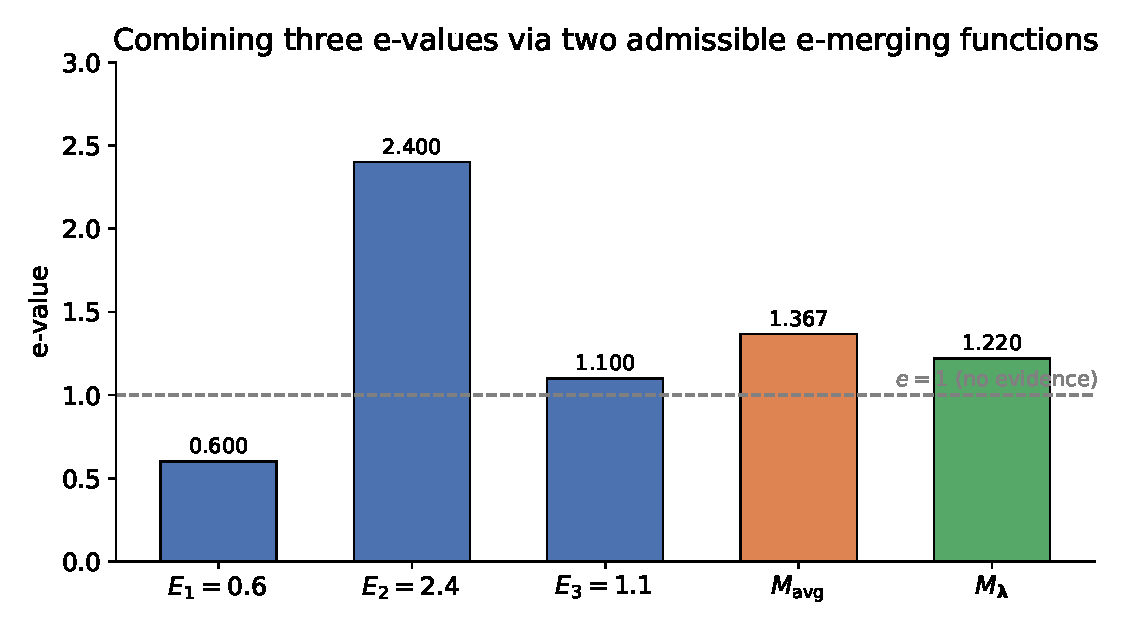
\includegraphics[width=0.8\textwidth]{fig_merging.pdf}
\end{center}
\vspace{-2mm}
{\footnotesize The three raw e-values (blue) and the two merged e-values: the plain average (orange) and the skeptical, intercept-shrunk average (green). The dashed line at $e=1$ marks ``no evidence.''}

\end{frame}

% ---------------------------------------------------------------------------
\begin{frame}[fragile]{Python: computing $\mathbb{M}_{\boldsymbol\lambda}$ e-merging functions}

\begin{lstlisting}
import numpy as np

def M_lambda(e, lam0, lam):
    """
    Admissible linear e-merging function M_lambda(e) = lam0 + sum_k lam_k * e_k.
    e    : array of K e-values
    lam0 : intercept weight  (skepticism toward e=1)
    lam  : array of K weights on the e-values
    Requires lam0 + sum(lam) == 1 and all weights >= 0  (lambda in Delta_{K+1}).
    """
    e = np.asarray(e, dtype=float)
    lam = np.asarray(lam, dtype=float)
    assert np.all(lam >= 0) and lam0 >= 0
    assert abs(lam0 + lam.sum() - 1.0) < 1e-9, "weights must lie in the simplex"
    return lam0 + np.dot(lam, e)

E = np.array([0.6, 2.4, 1.1])

# Rule 1: simple average
M_avg = M_lambda(E, lam0=0.0, lam=np.full(3, 1/3))

# Rule 2: skeptical weighted average
M_skep = M_lambda(E, lam0=0.4, lam=np.full(3, 0.2))

print(f"simple average   : {M_avg:.4f}")   # 1.3667
print(f"skeptical average: {M_skep:.4f}")  # 1.2200
\end{lstlisting}

\end{frame}

% ==========================================================================
\section{11.3 Cross-merging: e-value and p-value}

\begin{frame}{11.3 Intuition: combining evidence in different currencies}

Sometimes for the \emph{same} hypothesis $H$, you have one p-value $P$ (say, from a classical test) and one e-value $E$ (say, from a sequential or Bayesian analysis). You want one combined number that is still a valid p-value or e-value. There are four flavors, depending on:

\begin{itemize}
\item whether $P$ and $E$ are known/assumed to be \textbf{independent} (``i-'') or allowed to be \textbf{arbitrarily dependent} (``pe-''), and
\item whether the \textbf{output} should be a p-value (``/p'') or an e-value (``/e'').
\end{itemize}

This gives four cases: \textbf{i-pe/e}, \textbf{i-pe/p}, \textbf{pe/e}, \textbf{pe/p} (the chapter abbreviates ``pe'' in these names, e.g.\ just writing i/e, i/p, /e, /p). A \emph{combiner} is the function that performs this combination.

\end{frame}

% ---------------------------------------------------------------------------
\begin{frame}{Definition 11.4: combiners}

\begin{block}{Definition 11.4}
A function $f:[0,1]\times[0,\infty]\to[0,\infty]$ is an \textbf{i-pe/e combiner} if $f(P,E)$ is an e-value for any \emph{independent} p-value $P$ and e-value $E$ (for the same null), and $(p,e)\mapsto f(p,e)$ is decreasing in $p$ and increasing in $e$. Similarly define \textbf{i-pe/p}, \textbf{pe/p}, \textbf{pe/e} combiners, where ``i'' indicates the independence requirement, and ``p''/``e'' denote the output type. If the output is a p-value, the combiner is instead increasing in $p$ and decreasing in $e$.
\end{block}

\textbf{Monotonicity intuition.} A combiner producing an e-value should reward small $p$ (strong evidence) and large $e$ (strong evidence) with a \emph{larger} output; a combiner producing a p-value should do the opposite, since small p-values are the ones signaling evidence.

\end{frame}

% ---------------------------------------------------------------------------
\begin{frame}{Four natural combiners}

Let $h$ denote an admissible calibrator (a monotone function turning a p-value into an e-value, from Chapter 2).

\begin{block}{The four combiners}
\begin{itemize}
\item[\textbf{[ie]}] $C^{\mathrm{ie}}_h(p,e) = h(p)\,e$ \quad (returns $h(P)E$; convention $0\times\infty=\infty$). \hfill \emph{i-pe/e}
\item[\textbf{[ip]}] $C^{\mathrm{ip}}(p,e) = (p/e)\wedge 1$ \quad (returns $P/E$, capped at $1$). \hfill \emph{i-pe/p}
\item[\textbf{[e]}] $C^{\mathrm{e}}_{\lambda,h}(p,e) = \lambda\,h(p) + (1-\lambda)\,e$, $\lambda\in(0,1)$ \quad (average of two e-values $h(P)$ and $E$). \hfill \emph{pe/e}
\item[\textbf{[p]}] $C^{\mathrm{p}}(p,e) = \bigl(2\min(p,e^{-1})\bigr)\wedge 1$. \hfill \emph{pe/p}
\end{itemize}
\end{block}

\textbf{Note the pattern.} Combiners that assume \textbf{independence} ([ie], [ip]) can multiply/divide -- multiplication only controls the mean correctly under independence. Combiners valid under \textbf{arbitrary dependence} ([e], [p]) must instead use techniques (averaging, min with a factor of 2) that work no matter how $P$ and $E$ co-vary. $C^{\mathrm{e}}_{\lambda,h}$ and $C^{\mathrm{ie}}_h$ depend on the chosen calibrator $h$; $C^{\mathrm{ip}}$ and $C^{\mathrm{p}}$ do not -- mirroring how there are many admissible p-to-e calibrators but only one admissible e-to-p calibrator.

\end{frame}

% ---------------------------------------------------------------------------
\begin{frame}{Theorem 11.5 and the proof of the [ip] case}

\begin{block}{Theorem 11.5}
For an admissible calibrator $h$ and $\lambda\in(0,1)$: $C^{\mathrm{ie}}_h$ is an admissible i-pe/e combiner; $C^{\mathrm{ip}}$ is an admissible i-pe/p combiner; $C^{\mathrm e}_{\lambda,h}$ is an admissible pe/e combiner; $C^{\mathrm p}$ is an admissible pe/p combiner.
\end{block}

\textbf{Proof that $C^{\mathrm{ip}}(P,E)=P/E\wedge 1$ is a valid p-value (independent case), step by step.} For $t\in(0,1)$,
\[
\PP(C^{\mathrm{ip}}(P,E)\le t) = \PP(P/E\le t) = \PP(P \le tE) = \EE^\PP\bigl[\PP(P\le tE \mid E)\bigr] \le \EE^\PP[tE] \le t.
\]
\textbf{Reading each step:} (1) unwrap the cap (for $t<1$ it's inactive); (2) rearrange $P/E\le t \Leftrightarrow P\le tE$; (3) tower property, conditioning on $E$ and using independence of $P$ from $E$; (4) since $P$ is a valid p-value, $\PP(P\le s)\le s$ for any constant $s=tE$; (5) $\EE[E]\le 1$ since $E$ is an e-value. This chain of inequalities is exactly why we need \textbf{independence}: step (3) requires that conditioning on $E$ doesn't change the distribution of $P$.

\textbf{Admissibility} is proved by contradiction: assuming some combiner $f\le C^{\mathrm{ip}}$ but strictly smaller somewhere, one constructs an explicit two-point e-variable $E$ (mirroring the Lemma 11.2 technique) and a uniform $P$ that make $f(P,E)$ violate the p-value property -- contradicting validity of $f$.

\end{frame}

% ---------------------------------------------------------------------------
\begin{frame}{The quotient combiner and randomization (Example 11.6)}

$C^{\mathrm{ip}}(P,E) = P/E \wedge 1$ is called the \textbf{quotient combiner}. It is the workhorse of Section 11.4.

\begin{block}{Example 11.6: Randomization}
Let $E$ be an e-variable and $U\sim \mathrm{U}[0,1]$ independent of $E$. Applying the quotient combiner to $(U,E)$: $U/E$ is a valid p-value, and it satisfies $U/E \le 1/E$.
\end{block}

\textbf{Why this is interesting.} The map $e\mapsto (1/e)\wedge 1$ is the \emph{unique} admissible calibrator turning an e-value into a p-value (Chapter 2) -- yet here $U/E$ is a strictly \emph{smaller} (more significant) valid p-value than $1/E$ whenever $U<1$! This shows that allowing external randomization $U$ can improve upon the ``best'' deterministic e-to-p calibrator. The catch: $U/E$ requires generating extra randomness, which is impractical in general -- but becomes practical precisely when applied to an existing, already-random p-value $P$ independent of $E$, giving the quotient combiner $P/E$.

\end{frame}

% ---------------------------------------------------------------------------
\begin{frame}{When to prefer the quotient combiner? (rule of thumb)}

The quotient combiner $P/E$ is a natural tool for \textbf{meta-analysis} combining two independent datasets: one summarized as a p-value $P$, the other as an e-value $E$ (e.g., because it used optional stopping).

\begin{block}{Rule of thumb}
\begin{itemize}
\item If the two datasets are a priori \textbf{exchangeable} (similar power expected), prefer a symmetric method like \textbf{Fisher's combination} $P_{\mathrm F} := 1-\chi_4(-2\log(PP'))$ (using a second p-value $P'$ from the same data instead of $E$), since asymmetric rules like $P/E$ waste information when both datasets are equally informative.
\item If one dataset is \textbf{substantially more informative} (the ``primary'' dataset) than the other (the ``secondary'' dataset), and the p-value is computed on the more informative one, the quotient combiner $P/E$ can outperform Fisher's combination, and is asymptotically as efficient as the (infeasible) likelihood ratio test based on the full data, both as the significance level $\alpha\to0$ and as the secondary sample becomes negligible in size.
\end{itemize}
\end{block}

A stylized two-sample normal-mean example (comparing $\mathrm N(0,1)$ vs.\ $\mathrm N(\delta,1)$) confirms this numerically: when the secondary sample is small relative to the primary, $P/E$ nearly matches the optimal likelihood-ratio test and beats Fisher; when the two samples are balanced, Fisher edges out $P/E$, and both trail the likelihood ratio test slightly.

\end{frame}

% ==========================================================================
\section{11.4 E-values as weights}

\begin{frame}{11.4 Intuition: e-values as unnormalized weights}

\textbf{Setting.} We now have $K$ hypotheses $H_1,\dots,H_K$, each with a p-value $P_k$ \emph{and} an e-value $E_k$ (e.g., $E_k$ from a preliminary analysis, $P_k$ from an independent follow-up study; missing values default to $1$).

\textbf{Core idea.} Apply the quotient combiner \emph{coordinatewise}:
\[
P_k^* := (P_k/E_k)\wedge 1.
\]
\begin{itemize}
\item If $E_k > 1$ (evidence against $H_k$), then $P_k^* < P_k$ -- the reweighted p-value looks \emph{more} significant, i.e., the e-value strengthens the signal.
\item If $E_k < 1$ (no evidence against $H_k$), then $P_k^* > P_k$ -- the reweighted p-value looks \emph{less} significant.
\end{itemize}
So $E_k$ behaves exactly like a classical multiple-testing \textbf{weight}, except it need not be fixed in advance or normalized to sum to $K$ -- it can be random and data-dependent, and it can come from a completely separate analysis.

\end{frame}

% ---------------------------------------------------------------------------
\begin{frame}{Definition 11.9: the e-weighted p-value procedure}

\begin{block}{Definition 11.9 (ep-$\mathcal D$)}
Let p-$\mathcal D$ be any multiple testing procedure that takes p-values as input (e.g., Benjamini--Hochberg). The \textbf{e-weighted p-value procedure} ep-$\mathcal D$ proceeds as follows: for each $k\in\mathcal K=\{1,\dots,K\}$, compute the quotient combiner $P_k^* := (P_k/E_k)\wedge 1$, then supply the vector $\mathbf P^* = (P_1^*,\dots,P_K^*)$ to p-$\mathcal D$.
\end{block}

The chapter focuses on \textbf{ep-BH}: apply Definition 11.9 with p-$\mathcal D$ = the Benjamini--Hochberg (BH) procedure at level $\alpha$ (Chapter 9). Recall BH controls FDR at level $\alpha$ when the p-values are \textbf{PRDS} (a positive-dependence condition, Chapter 9's Definition 9.15).

\end{frame}

% ---------------------------------------------------------------------------
\begin{frame}{Theorem 11.10: FDR control for ep-BH}

Let $\mathcal N \subseteq \mathcal K$ index the true null hypotheses, and $K_0 = |\mathcal N|$.

\begin{block}{Theorem 11.10}
Suppose $\mathbf P$ is independent of $\mathbf E$ and $\mathbf P$ satisfies PRDS. Then the ep-BH procedure has $\mathrm{FDR} \le K_0\alpha/K$.
\end{block}

\textbf{Proof, step by step.}
\begin{enumerate}
\item \textbf{Condition on $\mathbf E$.} Since $\mathbf E \perp \mathbf P$, conditional on $\mathbf E=\mathbf e$, ep-BH is exactly a classical \textbf{weighted BH procedure} with (now-deterministic) weights $\mathbf e$ applied to the still-PRDS p-values $\mathbf P$.
\item \textbf{Apply the known weighted-BH FDR bound} (Ramdas et al., 2019, Thm.\ 1): for deterministic weights $\mathbf e$,
\[
\EE\left[\left.\frac{F_{\text{ep-}\mathcal D}}{R_{\text{ep-}\mathcal D}} \,\right|\, \mathbf E=\mathbf e\right] \le \frac{1}{K}\sum_{k\in\mathcal N} e_k\,\alpha.
\]
\item \textbf{Take expectation over $\mathbf E$ (tower property):}
\[
\mathrm{FDR}(\text{ep-BH}) = \EE\!\left[\frac{F_{\text{ep-}\mathcal D}}{R_{\text{ep-}\mathcal D}}\right] \le \EE\!\left[\frac{1}{K}\sum_{k\in\mathcal N} E_k\,\alpha\right] = \frac{\alpha}{K}\sum_{k\in\mathcal N}\EE[E_k] \le \frac{\alpha}{K}\sum_{k\in\mathcal N} 1 = \frac{K_0\alpha}{K}.
\]
The last inequality uses $\EE[E_k]\le 1$ for every $k\in\mathcal N$ (true nulls), since $E_k$ is a valid e-value there. $\blacksquare$
\end{enumerate}

\textbf{Remark.} Unlike classical weighted BH (fixed weights summing to $K$), the weights $E_k$ here are random, \emph{data-dependent}, and need not be normalized -- yet FDR control still holds, with \emph{no} assumption needed on the dependence structure of $\mathbf E$ itself.

\end{frame}

% ---------------------------------------------------------------------------
\begin{frame}{Concrete example: an e-value loosens a threshold}

Suppose hypothesis $H_k$ has raw p-value $P_k$ and e-value $E_k = 4.0$ (fairly strong independent evidence against $H_k$ from a preliminary study). Consider a nominal rejection threshold $\alpha = 0.05$ (e.g.\ the relevant BH cutoff at some step).

\textbf{Reweighted p-value.} $P_k^* = (P_k/E_k)\wedge 1 = P_k/4.0$ (as long as $P_k<4$, no capping). The testing rule ``reject if $P_k^* \le \alpha$'' becomes:
\[
\frac{P_k}{E_k} \le \alpha \quad\Longleftrightarrow\quad P_k \le \alpha \cdot E_k = 0.05 \times 4.0 = 0.20.
\]

\textbf{Conclusion.} The e-value $E_k=4.0$ \emph{loosens} the effective significance threshold on the raw p-value from $0.05$ to $0.20$ -- a fourfold increase in the region where $H_k$ gets rejected. Symmetrically, an e-value of $E_k = 0.25$ (weak preliminary evidence) would \emph{tighten} the threshold to $0.05\times0.25 = 0.0125$.

\vspace{2mm}
The next slide visualizes exactly this loosening/tightening effect across a range of weights.

\end{frame}

% ---------------------------------------------------------------------------
\begin{frame}{Figure: e-values as weights loosen/tighten thresholds}

\begin{center}
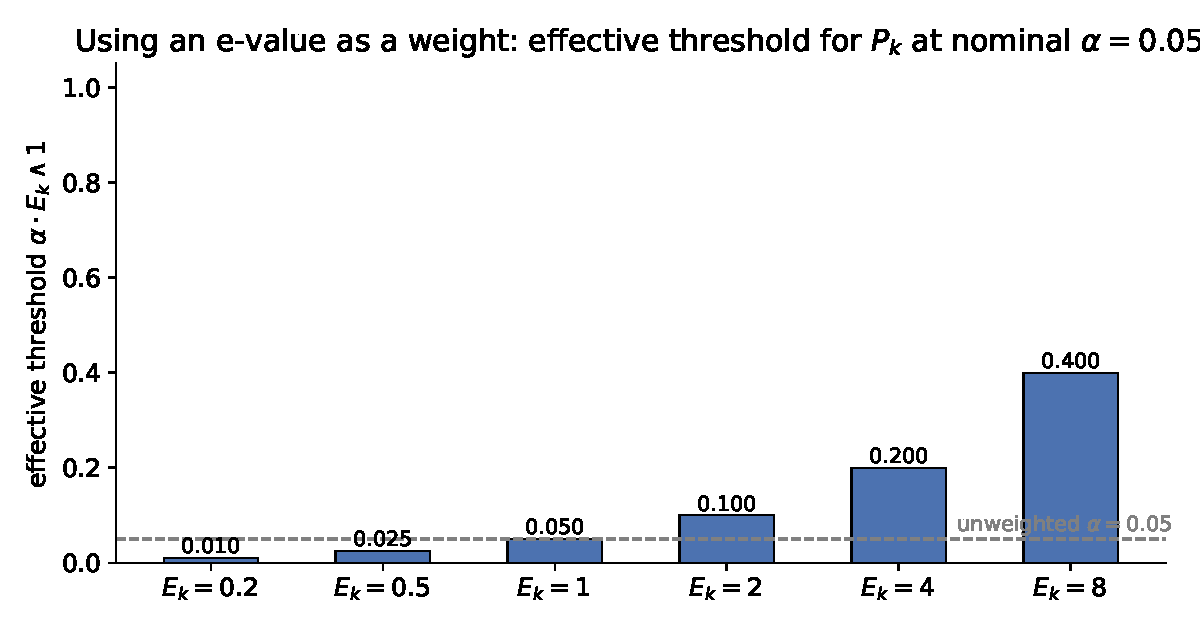
\includegraphics[width=0.85\textwidth]{fig_weights.pdf}
\end{center}
\vspace{-2mm}
{\footnotesize Effective rejection threshold $\alpha\cdot E_k \wedge 1$ for a toy panel of six tests with different e-value weights $E_k$, at nominal $\alpha=0.05$ (dashed line). Larger $E_k$ loosens the threshold; smaller $E_k$ tightens it.}

\end{frame}

% ---------------------------------------------------------------------------
\begin{frame}[fragile]{Python: the ep-BH procedure}

\begin{lstlisting}
import numpy as np

def ep_bh(p, e, alpha=0.05):
    """
    E-weighted Benjamini-Hochberg (ep-BH), Definition 11.9 + Theorem 11.10.
    p, e : arrays of K p-values and K e-values (same hypothesis order).
    Returns: boolean array of rejections.
    """
    p = np.asarray(p, dtype=float)
    e = np.asarray(e, dtype=float)
    K = len(p)

    # Step 1: quotient-combine each (p_k, e_k) pair into a reweighted p-value
    p_star = np.minimum(p / e, 1.0)

    # Step 2: run ordinary BH on the reweighted p-values p_star
    order = np.argsort(p_star)
    sorted_p = p_star[order]
    thresh = alpha * (np.arange(1, K + 1) / K)
    below = sorted_p <= thresh
    if not below.any():
        return np.zeros(K, dtype=bool)
    k_max = np.max(np.nonzero(below)[0])          # largest k with sorted_p[k] <= thresh[k]
    reject_sorted = np.zeros(K, dtype=bool)
    reject_sorted[: k_max + 1] = True
    reject = np.zeros(K, dtype=bool)
    reject[order] = reject_sorted
    return reject

# Toy illustration matching the threshold example: E_5 = 4.0 loosens things a lot
p = np.array([0.30, 0.02, 0.45, 0.60, 0.18])
e = np.array([1.00, 1.00, 1.00, 1.00, 4.00])
print("effective thresholds P_k/E_k at alpha=0.05:")
print(np.minimum(p / e, 1.0))
print("ep-BH rejections:", ep_bh(p, e, alpha=0.05))
\end{lstlisting}

\end{frame}

% ==========================================================================
\section{Summary}

\begin{frame}{Chapter summary}

\begin{itemize}
\item \textbf{11.1} Multi-marginal optimal transport duality (Lemma 11.1) is the technical engine: worst-case expectations under arbitrary dependence (sup over couplings) equal cheapest separable upper bounds (inf over coordinatewise functions).
\item \textbf{11.2} Using this duality plus a minimax swap and the $K=1$ Lemma 11.2, we proved Theorem 8.4: \emph{every} e-merging function is dominated by, and every admissible one equals, a linear combination $\mathbb M_{\boldsymbol\lambda}(\mathbf e) = \lambda_0+\sum_k\lambda_k e_k$ with $\boldsymbol\lambda\in\Delta_{K+1}$.
\item \textbf{11.3} Four natural combiners cross-merge a p-value and an e-value for the same hypothesis, all provably admissible (Theorem 11.5); the \textbf{quotient combiner} $P/E\wedge1$ is the most broadly useful, and is especially powerful for meta-analysis of an imbalanced pair of datasets.
\item \textbf{11.4} Plugging $P_k^*=(P_k/E_k)\wedge1$ into any p-value multiple-testing procedure (e.g.\ BH) turns e-values into valid, unnormalized, data-dependent \textbf{weights}: the ep-BH procedure controls FDR at $K_0\alpha/K$ whenever $\mathbf P\perp\mathbf E$ and $\mathbf P$ is PRDS -- with \emph{no} assumption on the dependence of $\mathbf E$.
\end{itemize}

\end{frame}

% ---------------------------------------------------------------------------
\begin{frame}{Bibliographical note}

\begin{itemize}
\item The optimal transport duality of Lemma 11.1 can be verified via Kellerer (1984); formula (11.1) appears in Rachev and R\"uschendorf (2006, Thm.\ 2.1.1) and R\"uschendorf (2013, Thm.\ 2.3). A standard textbook reference on optimal transport is Villani (2009).
\item Vovk and Wang (2021) identified all \emph{symmetric} admissible e-merging functions; the general (non-symmetric) case, Theorem 8.4 as presented here, is due to Wang (2025).
\item The content of Sections 11.3--11.4 is based on Ignatiadis et al.\ (2024b); the full proof of Theorem 11.5 is in their Appendix S1. Using deterministic weights for BH FDR control was studied by Benjamini and Hochberg (1997). The e-weighted BH procedure of Section 11.4 was introduced by Ignatiadis et al.\ (2024b), along with results for many other weighted procedures.
\end{itemize}

\end{frame}

\end{document}
